\section{Flip-Flops}

\subsection{D-Flip Flop}
	\begin{multicols}{3}
		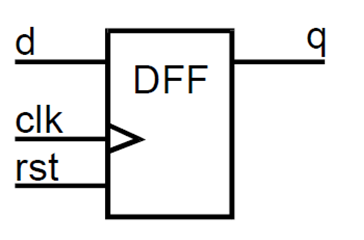
\includegraphics[width=0.2\textwidth]{pics/d-ff_sym}\\
		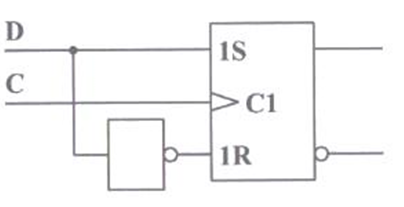
\includegraphics[width=0.2\textwidth]{pics/d-ff_sch}\\ 
		\begin{tabular}{|l|l|l|l|}
			%\hline
			%\multicolumn{4}{|l|}{Wahrheitstabelle}\\
			\hline
			nrst & d & clk & q\\
			\hline
			\hline
			0 & x & $\downarrow$ & speichern\\
			\hline
			0 & 0 & $\uparrow$ & 0 \\
			\hline
			1 & 1 & $\uparrow$ & 1(1)\\
			\hline
			1 & x & x & 0\\
			\hline
		\end{tabular}
	\end{multicols}
	
\subsection{RS-Flip Flop}
	\begin{multicols}{3}
		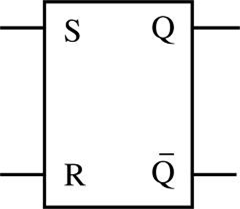
\includegraphics[width=0.2\textwidth]{pics/rs-ff_sym}\\	
		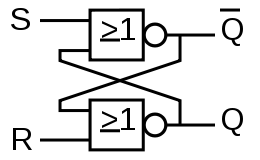
\includegraphics[width=0.2\textwidth]{pics/rs-ff_sch}\\
		\begin{tabular}{|l|l|l|l|}
			%\hline
			%\multicolumn{4}{|l|}{Wahrheitstabelle}\\
			\hline
			R & S & $Q_{n+1}$ & Kommentar\\
			\hline
			\hline
			0 & 0 & $Q_n$ & Speicherzustand \\
			\hline
			0 & 1 & 1 & Setzen \\
			\hline
			0 & 0 & 1 = $Q_n$ & Speichern(1)\\
			\hline
			1 & 1 & 0 & Zur�cksetzen\\
			\hline
			0 & 0 & 0 = $Q_n$ & Speichern(0)\\
			\hline
			1 & 1 & 0 & Undef. weil $Q_n = \bar{Q_n}$\\
			\hline
		\end{tabular}
	\end{multicols}


